\documentclass[10pt,a4paper]{article}
\usepackage[utf8]{inputenc}
\usepackage{amsmath}
\usepackage{amsfonts}
\usepackage{amssymb}
\usepackage{graphicx}
\usepackage{subcaption}
\graphicspath{ {./graphics/} }
\usepackage[colorlinks]{hyperref}
\usepackage{wrapfig}
\usepackage{float}
\usepackage{svg}
\usepackage[
backend=biber,
style=numeric,
sorting=ynt
]{biblatex}
\addbibresource{6D-Ae-report.bib}
\newcommand{\R}{\mathbb{R}}
\usepackage{blindtext}
\usepackage{xspace}
\usepackage{tikz}
\usepackage{pgf}
\usetikzlibrary{arrows,arrows.meta,shapes,shapes.multipart,shapes.geometric,shapes.misc,calc,positioning,decorations.pathreplacing,fit,backgrounds,positioning,calc}

\newcommand{\rot}{\ensuremath{\text{rot}\xspace}}
\newcommand{\trans}{\ensuremath{\text{trans}\xspace}}
\newcommand{\loss}{\ensuremath{\mathcal{L}_2}}


\begin{document}
  % Keine Seitenzahlen im Vorspann
  \pagestyle{empty}

  % Titelblatt der Arbeit
  \begin{titlepage}


 \begin{center} 
	{\Large\textbf{ 
		6D Pose Autoencoder
	}}
    \vspace{1cm}
    
    Project report Reconstructing and Understanding the 3D World\\
    at the IWR Institute in Heidelberg\\
    \vspace{5cm}
    submitted by\\
    \vspace{0.5cm}
	{\large\textbf{Till Bungert and Carsten Lüth}\\}
	\vspace{5cm}
	under the supervision of \\
	\vspace{0.5cm}
	{\large\textbf{Prof. Dr. Carsten Rother}\\}
	and\\
	{\large\textbf{Siva Karthik Mustikovela}\\}


    \vspace{3cm}
	{\Large\textbf{2018}}
	

	

  \end{center}
\end{titlepage}


  % Inhaltsverzeichnis
  \tableofcontents

\newpage

  % Ab sofort Seitenzahlen in der Kopfzeile anzeigen
  \pagestyle{headings}

\section{Introduction}\label{Introduction}
The determination of 6D poses for known objects is a very important subject for robotics and augmented reality. For example in robotics it is crucial to have an accurate understanding of the position of an object to interact with it in a meaningful way. Almost the same applies to augmented reality because to enhance any object by rendering information on its visible surface it is important to know the position of the said object.\\
There are many different ways to determine the 6D-Pose of a known object but in this work we will concentrate on a method which is based on the Augmented Autoencoder as designed by Martin Sundermeier et al. \cite{3D_Orientation_Learning}. This approach only uses RGB Images and does not require a big amount of labelled data to be trained because the autoencoder is tasked to reconstruct its input and not to predict the rotation and translation directly. This implicit learning makes it very robust against symmetries. Also in their paper they show that it can be fully trained on artificial generated images and also able to generalize to real images.\\
The general goal of this work is to use the augmented autoencoder to disentangle the rotation and translation information in the latent space with a novel training scheme as well as to give an theoretical motivation for the rotation learning of the network which gets backed up by our experiments. Due to the training schedule the training is self-supervised and completely conducted on rendered images.\\
All of our experiments are conducted on rendered data and also validated on rendered images. To render the images we used the open source renderer GLUMPY based on Numpy and OpenGL (XXXREFXX). \\  




\newpage

\section{Methods}\label{Methods}
In the following section we focus on the novel 6D-Autoencoder which is a new interpretation of the Augmented Autoencoder (AAE), introduced by Martin Sundermeier et Al. (XXXXXXXXX). First we introduce the concept of invariant latent space representations of an Autencoder via objective functions and then present a method to get the 6D-Pose based on the latent space representation.

\subsection{Autoencoder}\label{Autoencoder}
The original Autoencoder is a technique to map a high dimensional input ($x$), such as image or audio data, into a lower dimensional representation ($z$) ($D << N$) while maintaining the important information of its input. To achieve this the model which consists of an Encoder $\varphi$ and Decoder $\phi$ is tasked to reconstruct its input after passing it through a low dimensional bottleneck ($z$), where each of them is a general function approximator (neural network), resulting in the following objective function:
\begin{equation}
\min_{\varphi, \phi} L_{\text{rec}}(x, \phi(\varphi(x)))
\end{equation}
$L_{\text{rec}}$ can be any arbitrary distance metric on $\mathbb{R}^N$. 
A specialized form of the Autoencoder is the  Denoising Autoencoder. For this type of Autoencoder the input $x$ gets pertubed with random noise $\tilde{x} = f_{\text{noise}}(x) =x + \epsilon$ $\epsilon \sim \mathbb{P}_{\epsilon}$ while beeing tasked to reconstruct the unpertubed $x$. This results in the following objective function:
\begin{equation}
\min_{\varphi, \phi} L_{\text{rec}}(x, \phi(\varphi(f_{\text{noise}}(x) )))
\end{equation}
The trained model can be used to reconstruct unpertubed test images. But how is the latent space effected by this training schedule?
This question leads to the core assumption to create the AAE which gets motivated by a later experiment.
\paragraph{Hypothesis 1} To optimally reconstruct the unpertubed $x$ for the previously unseen test data the encoder should get in theory invariant to the pertubation. Meaning: Encoded Latent space representation of the input is invariant against the perturbation.\\
\paragraph{Regularized Autoencoder}
The regularized Autoencoder as described in XXXDeepLearningBookXXX is defined by an additional loss/ part of the objective function which is solely effected by the latent space representation. By adding this additional loss the latent space gains some desired properties such as a specific distribution with the Variational Autoencoder by using the KL-Divergence as latent loss.
Resulting objective function of a regularized Autoencoder:
\begin{equation}
\min_{\varphi, \phi} L_{\text{rec}}(x, \phi(\varphi(f(x) ))) + L_{\text{lat}}(\varphi(f(x)))
\end{equation}
$f$ can be any arbitrary augmentation or just the identity.


\subsection{6D Pose Autoencoder}\label{6D Pose Autoencoder}
\begin{figure}[htb]
    \centering
    \begin{tikzpicture}[
    coder/.style = {trapezium, trapezium angle=70, minimum width=20mm, draw, thick},
    trapezium stretches=true,
    vector/.style = {rectangle split, rounded corners=1mm, rectangle split
        parts=2, thick, draw, inner ysep=5mm, rectangle split part
    fill={lime!40, orange!40}},
    mat/.style = {inner sep=0mm, column sep=0mm,nodes=draw},
    img/.style = {inner sep=0, outer sep=-3mm},
    fat arrow/.style = {double arrow, thick, draw, anchor=mid, align=center,
    text depth=-0.5pt, text width = 1.5cm, text = black},
    node distance = 5mm
    ]
    \node [vector] (z) {$z_1$ \nodepart{second} $z_2$};
    \node [coder, fill=black!20, shape border rotate=270, left=of z] (E) {Encoder};
    \matrix [row sep=2mm, right= of z]
    {
        \node [coder, fill=lime!40, shape border rotate=90] (D1) {Decoder}; & \\
        \node [coder, fill=orange!40, shape border rotate=90] (D2) {Decoder}; & \\
    };
\draw [->, thick] (E.east)
    -- ($(0,0)!($(0,0)!($(z.north west)!0.5!(z.west)$)!(0,1) +
    (0,0)!($($(z.north
    west)!0.5!(z.west)$)!0.5!(E.east)$)!(1,0)$)!(1,0)+(0,0)!(E.east)!(0,1)$)
    -- ($(0,0)!($(z.north west)!0.5!(z.west)$)!(0,1) + (0,0)!($($(z.north
    west)!0.5!(z.west)$)!0.5!(E.east)$)!(1,0)$)
    -> ($(z.north west)!0.5!(z.west)$);

\draw [->, thick] (E.east)
    -- ($(0,0)!($(0,0)!($(z.south west)!0.5!(z.west)$)!(0,1) +
    (0,0)!($($(z.south
    west)!0.5!(z.west)$)!0.5!(E.east)$)!(1,0)$)!(1,0)+(0,0)!(E.east)!(0,1)$)
    -- ($(0,0)!($(z.south west)!0.5!(z.west)$)!(0,1) + (0,0)!($($(z.south
    west)!0.5!(z.west)$)!0.5!(E.east)$)!(1,0)$)
    -> ($(z.south west)!0.5!(z.west)$);

\draw [->, thick] ($(z.north east)!0.5!(z.east)$) -- ($(0,0)!($(z.north
    east)!0.5!(z.east)$)!(0,1) + (0,0)!($($(z.north
    east)!0.5!(z.east)$)!0.5!(D1.west)$)!(1,0)$) -- ($(0,0)!($(0,0)!($(z.north
    east)!0.5!(z.east)$)!(0,1) + (0,0)!($($(z.north
    east)!0.5!(z.east)$)!0.5!(D1.west)$)!(1,0)$)!(1,0)+(0,0)!(D1.west)!(0,1)$)
    -> (D1.west);

\draw [->, thick] ($(z.south east)!0.5!(z.east)$)
    -- ($(0,0)!($(z.south east)!0.5!(z.east)$)!(0,1)
    + (0,0)!($($(z.south east)!0.5!(z.east)$)!0.5!(D2.west)$)!(1,0)$)
    -- ($(0,0)!($(0,0)!($(z.south east)!0.5!(z.east)$)!(0,1)
    + (0,0)!($($(z.south east)!0.5!(z.east)$)!0.5!(D2.west)$)!(1,0)$)!(1,0)
    + (0,0)!(D2.west)!(0,1)$)
    -> (D2.west);

\node [img, left= of E] (in) {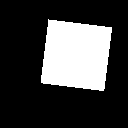
\includegraphics[width=20mm]{./input.png}};
\node [img, right= of D1] (o1) {
\includegraphics[width=20mm]{./output1.png}};
\node [img, right= of D2] (o2) {
\includegraphics[width=20mm]{./output2.png}};
\node [fat arrow, right= of o1] (l1) {$\loss$};
\node [fat arrow, right= of o2] (l2) {$\loss$};
\node [img, right= of l1] (t1) {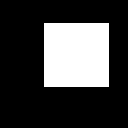
\includegraphics[width=20mm]{./target1.png}};
\node [img, right= of l2] (t2) {
\includegraphics[width=20mm]{./target2.png}};

\end{tikzpicture}

    \caption{The Model}
\end{figure}
The motivation of the 6D-Pose-Autoencoder is to get two latent space $z_{\rot}$ and $z_{\trans}$ from which the 6D pose comprised of rotation and translation can be read out separately.
Therefore $z_{\rot}$ encodes the orientation and should be invariant against translation while $z_{\text{trans}}$ encodes the translation while being invariant for rotations. This is done by taking two separate Augmented Autoencoder, one for the translation and one for the rotation. They receive the same input but are trained to reconstruct differently augmented versions of the input $x_{\text{rot}}$ and $x_{\text{trans}}$ . The training schedule is inspired by \textbf{Hypothesis 1}.
This is achieved by applying random augmentations $f_{\text{aug}}$ comprised of a $f_{\trans}$ and $f_{\rot}$ on the input $x$. 
\begin{equation}
 \begin{aligned}
\tilde{x} = &f_{\text{aug}} (x) = (f_{\trans} \circ f_{\rot} ) (x) \\
x_{\rot} =&f_{\rot} (x) \\
x_{\trans} =&f_{\trans} (x) \\
\hat{x}_{\rot} =& (\phi_{\rot} \circ \varphi_{\rot} \circ f_{\text{aug}}) (x) \\
\hat{x}_{\trans} = &(\phi_{\trans} \circ \varphi_{\trans} \circ f_{\text{aug}}) (x)
\end{aligned}
\end{equation}
The objective function of the system thereby is:
\begin{equation}
 \begin{aligned}
\min_{\varphi_{\rot}, \phi_{\rot}}  L_{\text{rec}}(x_{\rot}, \phi_{\rot}(\varphi_{\rot}(f_{\text{aug}}(x) ))) \\
\min_{\varphi_{\trans}, \phi_{\trans}}  L_{\text{rec}}(x_{\trans}, \phi_{\trans}(\varphi_{\trans}(f_{\text{aug}}(x) ))) 
\end{aligned}
\end{equation}
For the final model $\varphi_{\rot} = \varphi_{\rot}` \circ \varphi$ and $\varphi_{\trans}= \varphi_{\trans}` \circ \varphi$ so they are encoded by the same encoder and $z_{\rot}$ and $z_{\trans}$ are just created by a split int its latent space. The complete architecture can be seen in figure XXXXX.
\paragraph{Rotation} A rotation in one axis can be represented by a circle in $\mathbb{C}$ parametrized by $\theta \in [0, 2 \pi]$ with $\exp(i \theta)$ the choice  is near to define $z_{\rot} \in \mathbb{R}^2$ and using as $L_{\text{lat}}(z) = \text{abs} (||z_{\rot}||_2^2 -1)$ which forces the encoded $z_{\rot}$ to be on the unity circle. \\ 
Rotations with three axes can be represented in a similar manner as hyper sphere in $\mathbb{H}$. So for three rotational axes we defined $z_{\rot}$ to be in $\mathbb{R}^4$ which is a generalization of $\mathbb{H}$ with the same latent loss as stated above.\\
\paragraph{Translation} The translation of the object is a simple regression problem with uncorrelated factors. So we chose the simplest method to obtain a dense feature space in $z_{\trans} \in \mathbb{R}^3$ by taking as $L_{\text{lat}}(z) = z_{\trans}^2$. This is done because traditional autoencoders on mnist for example often have translations as single latent dimensions. An interesting fact is that the $z$ or depth axis could also be parametrized by scale so for objects with similar shape but different scales there would also be some ambiguities. 

\newpage
\subsection{Codebook}\label{Codebook}
The 6D-AE is after training able to extract the 3D orientation in $z_{\rot}$ and the translation in $z_{\trans}$. The clarity, orientation and translations of the reconstructions are a first indicator of the quality of the encodings. To extract the orientation and translation from the latent space representations we create a codebook for both rotation and translation.\\
This is done in the following way:
\begin{enumerate}
\item Render synthetic objects with known translation and rotation\\
\item Create a codebook by encoding the rendered images to $z_{\rot}\in \mathbb{R}^{O-1)}$ and $z_{\trans} \in \mathbb{R}^3$ where each of those belongs to a specific rotation and translation with respect to the camera
\end{enumerate}
The next step is to utilize the K-Nearest-Neighbour algorithm separately on the two latent space representations of the test images with unknown labels compared to the codebook with known labels.\\
The Distance metric used for the rotations $z_{\rot}$ is the cosine similarity. This is done because we initially made the assumption that our representations lie in a hyper sphere with unit distance from the origin.
\begin{equation}
\cos_i = \dfrac{z_i \cdot z_{\text{test}}}{ \vert\vert  z_i \vert \vert \cdot \vert \vert z_{\text{test}} \vert \vert }
\end{equation}
For the translation the euclidean distance was chosen as distance metric to determine the next nearest neighbours.



\newpage
\section{Evalutation}\label{Evaluation}
In the following section we present our results to prove our concepts presented in the chapter methods \ref{Methods}.
XXXXXXXXXXXXXXXXXXXXXX
\subsection{2D Square in 3D Space}\label{Square}
The goal of this experiment was to reproduce the results of Martin Sundermayer et al. in XXXXXXX with the AAE and show that the rotation and translation can be disentangled in principle with this very easy object. $z_{\rot}$ was defined to be in in $\mathbb{R}^2$ representing $\mathbb{C}$ as described in chapter \ref{Methods} due to the single rotation axis of the object. Due to the two perpendicular axes of symmetry the square posses we should see a shifted and cosine function with the frequency $f = \dfrac{4}{2 \pi}$, because the square appears exactly the same after a rotation of $\dfrac{\pi}{2}i$. \\
The second part was to show that the translation could be extracted from the latent space representation $z_{\trans}$ and that different rotations have neglegible effect on it. The resulting plot for the correlation between $z_{\rot}$ and the rotation $\varphi$ as well as $z_{\trans}$ and the translation can be seen in figure XXXXXXXX.
\newpage
\subsection{3D Cube}\label{Cube}
In this experiment we wanted to expand our predictions to a more complex case by taking the next complex object from the 2D square in 3D, namely the 3D cube. the 3D cube can be rotated in 2 axes due to trivial reasons of symmetry which leads to the conclusion that the rotations should be able to be represented by a hyper-sphere in 3 dimensions. So $z_{\rot}$ was chosen to be element of $\mathbb{R}^3$. The correlations between $z_{\rot}$ and the rotations as well as $z_{\trans}$ and the translation can be seen in figure XXXXXXXX.
Due to the more complex nature of the correlations in this case we also used the codebook created with our fully trained model to show the capabilty of this architecture. The resulting errors can be seen in table XXXXXXXXXXXX.
\newpage
\subsection{Line Mod}
Our final experiments were conducted on the LINE MOD created by Stefan Hinterstoisser \cite{LINEMOD} to evaluate the capability of the 6D Pose AE on two very different objects. Namely the cat and the egg-box where the model should show that it can be used on cases with no symmetry like the cat as well as many symmetries such as the egg-box in general cases with all 3 rotations and thereby the resulting latent space representations $z_{\rot} \in \mathbb{R}^4$. Ideally the resulting model can be used to determine the 3 rotation values as well as to be able to detect rotation symmetries like in the egg box by itself making it very robust against ambiguities. 
\subsubsection{Cat}
As mentioned before the cat object of the line mod dataset has no symmetries which makes it a good proof of concept to show that the 3 rotations can be displayed by the network on the unity sphere in $\mathbb{R}^N$ which makes it a generalization of the hamiltonians $\mathbb{H}$. Also this allows us to test whether this assumption really fits by calculating the resulting $i, j \text{ and } k$ of two rotations and applying (multiplicating) them onto each other. The resulting quaternion is then compared with the quaternion which we get by computing the quaternion we get from the network predicted.

\subsubsection{Egg Box}
The Egg Box has many symmetries and the ideal case is that the network learns these symmetries by changing the frequencies of the latent space repetitions in $z_{\rot}$
\newpage
\section{Conclusion}
The general concept of this work namely the split in rotational latent space $z_{\rot}$ and translational latent space $z_{\trans}$ of the augmented autoencoder was shown to work  extremely well by restricting the size of the latent space in experiments A TO B.\\
We were able to extract the 3D orientation as well as the 3D rotation with regard to the camera of the object with the codebook.\\
\\
The connection between $N$-dimensional rotations and the $N-1$-dimensional unity sphere was shown to be appropriate and used to minimize the size of the latent space in the experiment SQUARE and CAT\\
\\
In general this model thereby allows a more accurate estimation of the 3D translation than the model presented by martin sundermeier et. al. .
It is also easily able to detect on which object the network is basing its prediction of the codebook by checking the translation reconstruction in case of misspredictions or multiple objects of the same class.\\

 

\section{Sources}\label{Sources}
\printbibliography*



\end{document}
